\documentclass{homework}
\usepackage{xcolor}
\usepackage{nicematrix}
\usepackage{booktabs}
\usepackage{enumitem}
\usepackage{caption}
\usepackage{subcaption}
\usepackage{leftidx}
\usepackage{mathrsfs}
\usepackage{pgfplots, pgfplotstable}

\NiceMatrixOptions{cell-space-limits = 1pt}

\title{Simulation and Modeling I, Assignment 3}
\author{
  Dmitrii, Maksimov\\
  \texttt{dmitrii.maksimov@fau.de}
  \and
  Priyanka, Muddarla\\
  \texttt{priyanka.muddarla@fau.de}
  \and
  Susmitha, Palla\\
  \texttt{susmitha.palla@fau.de}
  \and
  Bhaskar Jyoti, Gogoi\\
  \texttt{bhaskar.j.gogoi@fau.de}
}


\begin{document}

\maketitle

\exercise
Use Little’s Law and the provided formulas and your solutions for Assignment 2 Problem 4 to provide estimations for the following scenarios:
\begin{enumerate}[label=(\alph*)]
	\item Consider a simple M/M/1 queue with exponentially distributed interarrival times with rate $\lambda=0.75$ and exponentially distributed services times with rate $\mu=1.0$.

Calculate the average values for:
\begin{itemize}
	\item utilization (U) $U = \frac{\lambda}{\mu}=0.75$
	\item number of custtomers in the system (N) $N = \frac{U}{1 - U} = 3$
	\item throughput(X)

	Since $U < 1$: $X = m\cdot U\cdot \mu$, where $m$ - the number of servers in a system = 1 $\Rightarrow X=0.75$
	\item time spent in the system (D), using Little's Law $D = \frac{N}{X} = 4$
\end{itemize}
	\item How do the measures D and N change for a simple M/D/1 queue with the same arrival rate and identical mean service time as the M/M/1 queue above? 
	
	\begin{itemize}
	\item Let $S$ - the service time, then $D = W + E[S] = \frac{U(c_s^2 + 1)}{2\mu(1-U)} + {\mu}$. \newline Since, $c_s = 0$: $D = \frac{U}{2\mu(1-U)} + \mu =  2.5$.
	\item $N=D\cdot X=1.875$
	\end{itemize}
	
\end{enumerate}
\exercise Extend the model so that
\begin{enumerate}[label=(\alph*)]
	\item the simulation run stops after a specified number of customers have been served(instead of stopping after a specified stop time)!
	\item the statistical data for
	\begin{enumerate}[label=(\roman*)]
		\item $N(t)$: number of customers in system at time t
		\begin{figure}[hbt!]
		     \centering
		     \begin{subfigure}[hbt!]{0.4\textwidth}
			\centering
			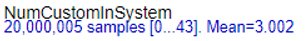
\includegraphics[width=\textwidth]{N_MM1.png}
			\caption{for an M/M/1}
		     \end{subfigure}
		     \hfill
		     \begin{subfigure}[hbt!]{0.4\textwidth}
		         \centering
		         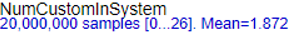
\includegraphics[width=\textwidth]{N_MD1.png}
		         \caption{for an M/D/1}
		     \end{subfigure}
		        \caption{Expectation of N(t)}
		\end{figure}
		\item $D(i)$: time spent in system by $i-th$ customer
		\begin{figure}[hbt!]
		     \centering
		     \begin{subfigure}[hbt!]{0.4\textwidth}
			\centering
			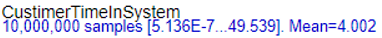
\includegraphics[width=\textwidth]{D_MM1.png}
			\caption{for an M/M/1}
		     \end{subfigure}
		     \hfill
		     \begin{subfigure}[hbt!]{0.4\textwidth}
		         \centering
		         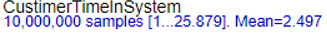
\includegraphics[width=\textwidth]{D_MD1.png}
		         \caption{for an M/D/1}
		     \end{subfigure}
		        \caption{Expectation of D(i)}
		\end{figure}

	As we can see calculatios are approximately equal.
	\end{enumerate}
	\item the statistical data for
	\begin{enumerate}[label=(\roman*)]
		\item $B(t)$ utilization
		\begin{figure}[hbt!]
		     \centering
		     \begin{subfigure}[hbt!]{0.4\textwidth}
			\centering
			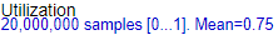
\includegraphics[width=\textwidth]{U_MM1.png}
			\caption{for an M/M/1}
		     \end{subfigure}
		     \hfill
		     \begin{subfigure}[hbt!]{0.4\textwidth}
		         \centering
		         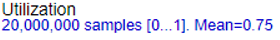
\includegraphics[width=\textwidth]{U_MD1.png}
		         \caption{for an M/D/1}
		     \end{subfigure}
		        \caption{Expectation of B(t)}
		\end{figure}
		\item $X(t)$: number of customers served per time unit
		\begin{figure}[hbt!]
		     \centering
		     \begin{subfigure}[hbt!]{0.4\textwidth}
			\centering
			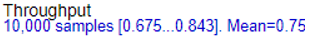
\includegraphics[width=\textwidth]{X_MM1.png}
			\caption{for an M/M/1}
		     \end{subfigure}
		     \hfill
		     \begin{subfigure}[hbt!]{0.4\textwidth}
		         \centering
		         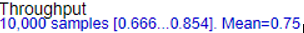
\includegraphics[width=\textwidth]{X_MD1.png}
		         \caption{for an M/D/1}
		     \end{subfigure}
		        \caption{Expectation of X(t)}
		\end{figure}

	As we can see calculatios are equal.
	\end{enumerate}
	\item What is your (estimate of the) coefficient of variation of the time spent in the system for the M/M/1 and the M/D/1? Make a conclusion on how this random variable might be distributed for both cases!
	\newpage
	 Coefficient of variation: $C_X = \frac{\sigma_X}{E[X]}$
	\begin{itemize}
		\item M/M/1
		\begin{figure}[hbt!]
			\centering
			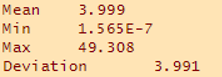
\includegraphics[width=0.3\textwidth]{O_MM1.png}
			\caption{Statistics of M/M/1}
		\end{figure}

		Hence, $C_X \approx 1$. It's obvious, since this is exponential distribution.
		\item M/D/1
		\begin{figure}[hbt!]
			\centering
			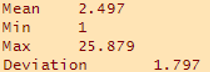
\includegraphics[width=0.3\textwidth]{O_MD1.png}
			\caption{Statistics of M/D/1}
		\end{figure}

		Hence, $C_X \approx 0.72$.
		Taking into account that we are in Erlangen let it be the Erlang distribution(joke). Exponential distrubition is a special case of the Erlang distribution with $k=1$. Coefficient of variation of Erlang distribution: $C = \frac{1}{\sqrt{k}}$. Hence, it seems to be the Erlang distribution witk k = 2.
	\end{itemize}
\end{enumerate}


\end{document}